\section{Storia} % (fold)
	\label{sec:storia}
	
	\begin{frame}[t]\frametitle{Storia}
		\begin{itemize}
			\item 1897 $\longrightarrow$ \href{http://www.wired.it/scienza/energia/2014/04/30/la-scoperta-dellelettrone/}{Scoperta dell'elettrone} da parte di Thompson 
			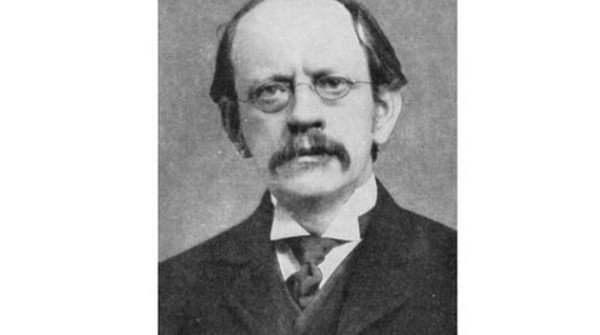
\includegraphics[width=4cm]{./img/thompson.jpg}
			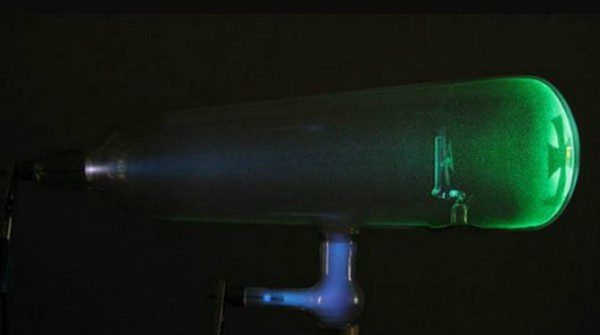
\includegraphics[width=4cm]{./img/tubo.jpg}
			\pause
			\item 1900  $\longrightarrow$ Primo modello di metallo proposto da Paul Drude (1863 – 1906) con l'atomo a panettone
			
			%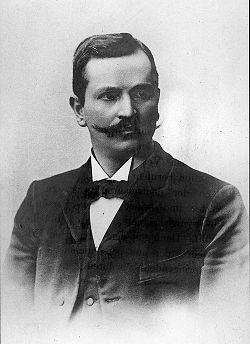
\includegraphics[width=2cm]{./img/Drude.jpg}
			\pause
			\item 1911  $\longrightarrow$ Atomo di Ernest Rutherford ( 1871 – 1937)
		\end{itemize}
	\end{frame}
	\note{2 parole sul modello a panettone e su come si sono accorti che questo non funzionava grazie allo scattering di particelle alfa elio \href{http://www.dmf.unicatt.it/~sangalet/PLS/Buone_pratiche/Esperimento_Rutherford.pdf}{fonte} 1/8000 falliva la previsione, figata che è la scienza, il modello di drude è quanto andremo noi a vedere anche se precisiamo già da ora che è falso ma rende molto bene l'idea.}

	\begin{frame}[c]\frametitle{Atomo di Rutherford}
	    
		\centering 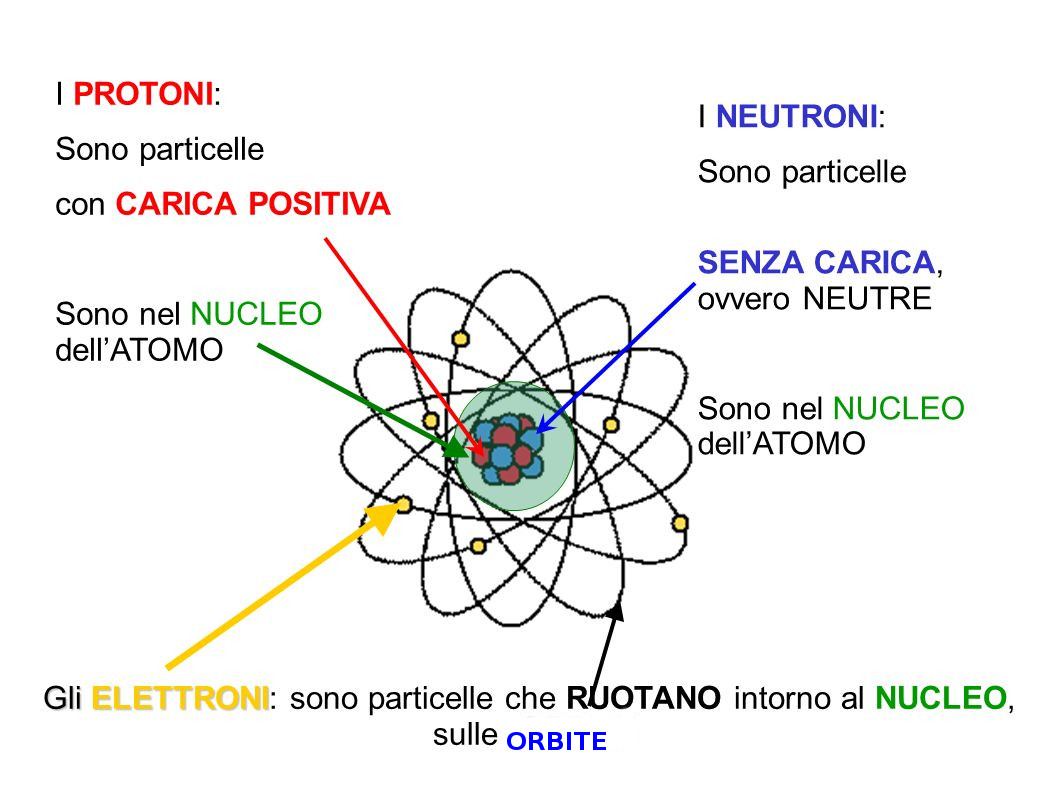
\includegraphics[width=9cm]{./img/atomo.jpg}

	\end{frame}
	\note{elettroni legati!!!!}

	\begin{frame}[c]\frametitle{Atomo di rame}
	    \begin{columns}
			\begin{column}{0.4\textwidth}
				\centering 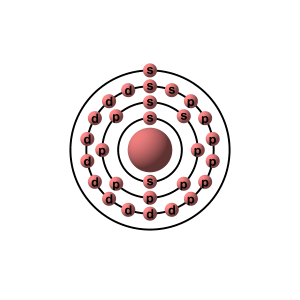
\includegraphics[width=5cm]{./img/rame.png}
			\end{column}
			\begin{column}{0.4\textwidth}
				\begin{itemize}
					\item Nucleo
					\begin{itemize}
						\item Neutroni
						\item Protoni
					\end{itemize}
					\item Elettroni
				\end{itemize}

				\vspace{0.5cm}
				
				$\longrightarrow$ Elettroni e ione!!

			\end{column}
		\end{columns}
	
	\end{frame}

	% section storia (end)

	\section{Il modello} % (fold)
	\label{sec:il_modello}
		\begin{frame}[c]\frametitle{Il metallo}
		    
		Cosa accade quando avviciniamo molti atomi?
		\centering 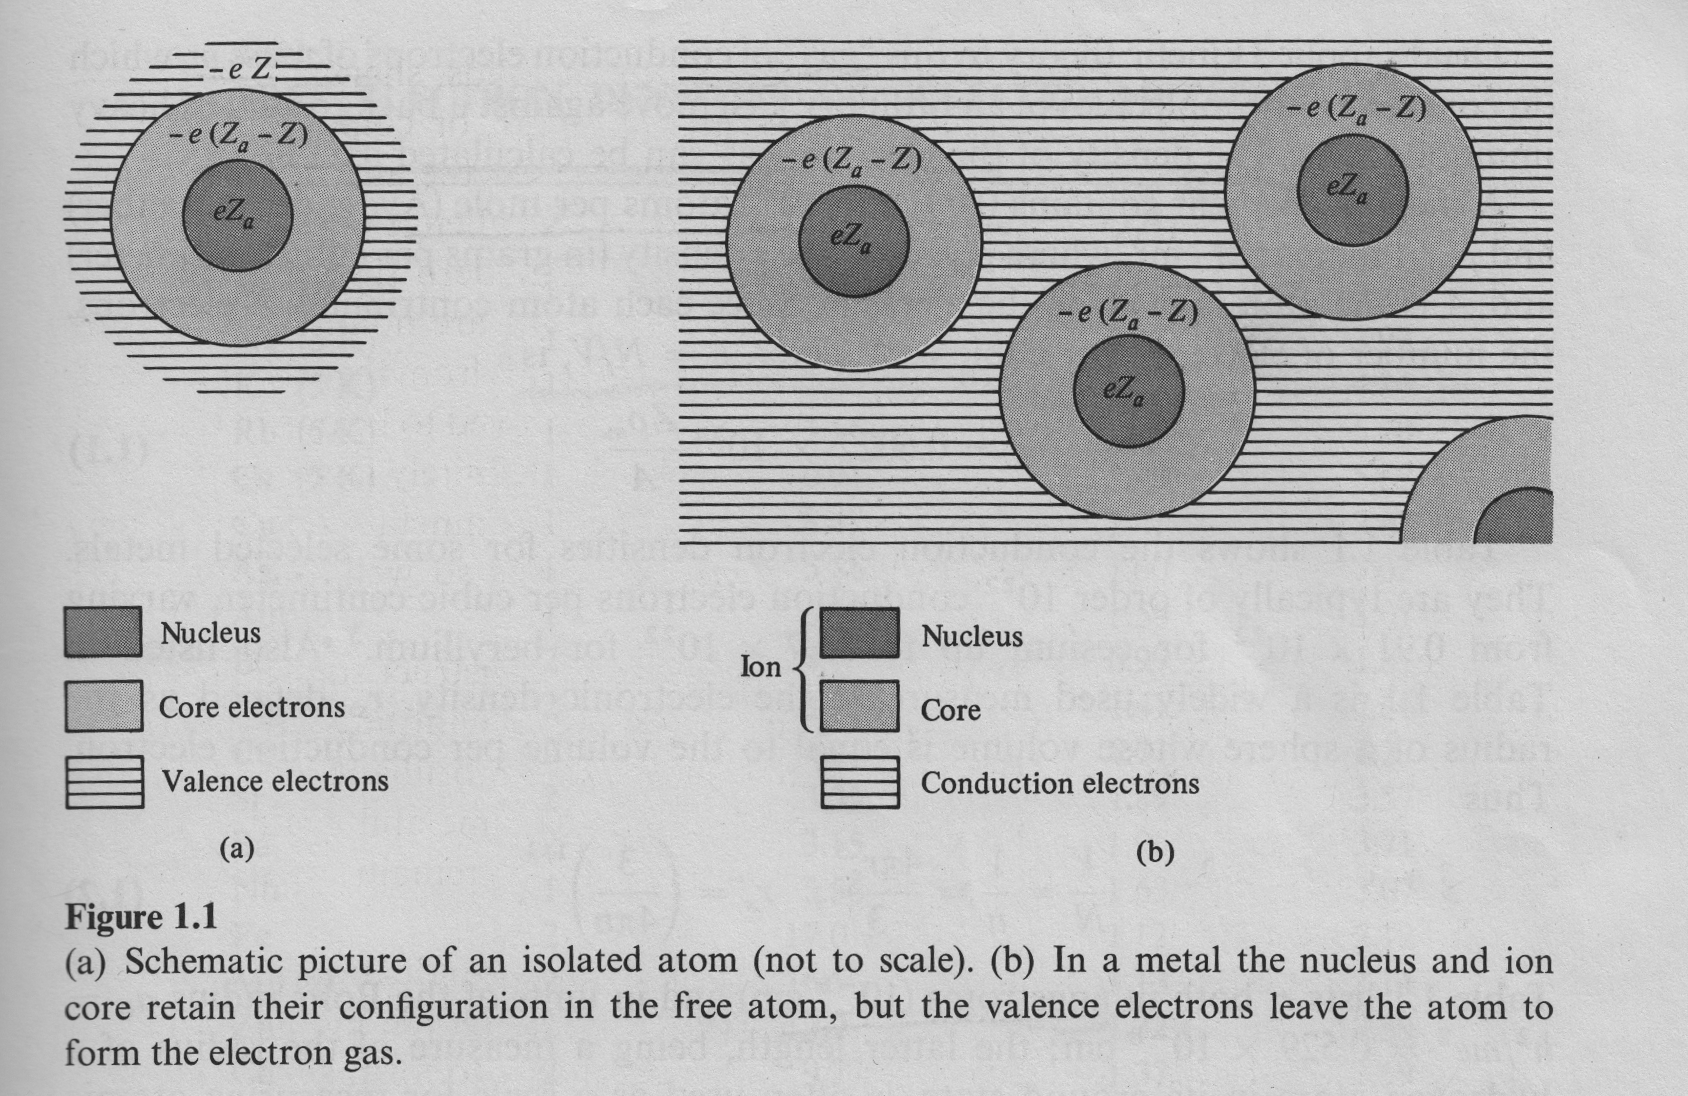
\includegraphics[width=9cm]{./img/model.png}
		
		\end{frame}

		\note{gli elettoni si muovono a caso ma la velocità media è nulla, non interagiscono fra di loro, interagiscono solo con gli atomi}
		
		\begin{frame}[c]\frametitle{Se applichiamo una differenza di potenziale?}
			\begin{columns}
				\begin{column}{0.4\textwidth}
					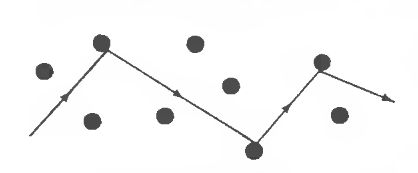
\includegraphics[width=4cm]{./img/path.png}
				\end{column}
				\begin{column}{0.7\textwidth}

					$\longrightarrow$ $V(x)$ Potenziale\\
					$\longrightarrow$ $E(x)$ Campo Elettrico
					\[
					 E (x) = - \frac{V(x1)-V(x2)}{\Delta x}
					\]
					\[
					 F \left(x\right) = q \left(x\right) E(x)
					\]

				\end{column}
			\end{columns}
			--nota slide per 3--
		\end{frame}
		\note{gli elettroni cominciano a muoversi con una direzione preferenziale }

		\begin{frame}[c]\frametitle{Disclaimer}
		    
		\begin{center}
			Attenzione!!
		\end{center}
		Questo modello funziona (ovvero fa buone previsioni) su alcuni conduttori e in condizioni normali ma è FALSO, la resitenza NON è data dagli urti degli atomi con i nuclei ma fenomeni ben più complicati che richiedono conoscenze di M.Q. e di matematica non banali per essere descritti e che pertanto non andiamo ad affrontare. Abbiamo scelto questo modello perché ci è sembrato, dal punto di vista didattico il miglior modo per introdurre l'argomento.		
		\end{frame}
	% section il_modello (end)

	\section{La resistenza} % (fold)
	\label{sec:la_resistenza}
		\begin{frame}[c]\frametitle{Come si misura e come si calcola}
		    \begin{columns}
		    	\begin{column}{0.4\textwidth}
		    		\[
		    		 R = \frac{\ro L}{A}
		    		\]
		    		
		    	\end{column}
		    \end{columns}
		
		
		\end{frame}
	
	% section la_resistenza (end)

	\section{Storia} % (fold)
		\label{sec:il_formalismo_di_fourier}
	
		\begin{frame}[c]\frametitle{La serie di Fourier}

		\begin{block}{Lo sviluppo in serie}
			\begin{equation}
		    	\label{eq:serie_di_fourier}
				f\left(t\right)=\sum_{n=-\infty}^{\infty} C_n e^{i n \omega t}
			\end{equation}
		\end{block}
		\pause
		\begin{block}{Il valore dei coefficiente coefficineti}
			\begin{equation}
			    \label{eq:coefficienti}
					C_n= \frac{1}{T} \int_{-\frac{T}{2}}^{\frac{T}{2}} f\left(t\right) e^{-i n \omega t} \,dt
			\end{equation}
		\end{block}

		\end{frame}
		
		\begin{frame}{La trasformata di Fourier}
		
			\begin{block}{La Trasformata}
				\begin{equation}
					\mathcal{F} \left [ f \left ( t\right)\right ] =\frac{1}{\sqrt{2\pi}} \int_{-\infty}^{\infty} f \left ( t \right ) e^{-i \omega t} \, dt
				\end{equation}		
			\end{block}	

			\pause
			
			\begin{block}{L'anti trasformata}
				\begin{equation}
				    \label{eq:antitrasformata}
					\mathcal{F}^{-1} \left [ F \left ( \omega \right)\right ] =\frac{1}{\sqrt{2\pi}} \int_{-\infty}^{\infty} F \left ( \omega \right ) e^{i \omega t} \, d\omega
				\end{equation}
			\end{block}
		
		\end{frame}
		
	%end sec il formalismo

	\section{Tipologie di filtri} % (fold)
	\label{sec:tipologie_costruttive_di_filtri}
		\subsection{Metodo di trattamento dei dati} % (fold)
		\label{sub:metodo_di_trattamento_dei_dati}

		\begin{frame}[c]\frametitle{Filtri analogici}
		    
				sfruttano le particolari funzioni di trasferimento dei loro componenti per di svolgere la funzione matematica cercata
				\pause
				\begin{block}{Passivi}
					Non possiedono elementi in grado di dare potenza al segnale(Transisor, Operazionali)
				\end{block}
				\pause
				\begin{block}{Attivi}
					Possono dare potenza al segnale assorbendola da fonti esterne ovviamente
				\end{block}
		
		\end{frame}

		\begin{frame}[c]\frametitle{Filtri digitali}

			Prevedono la digitalizzazione del segnale e una conseguente elaborazione dei dati raccolti attraverso particolari algoritmi.
			\begin{itemize}
				\pause
				\item Non prevedono la suddivisione precedente
				\pause
				\item Sono molto sensibili alla capacità di calcolo del microporcessore
			\end{itemize}

		\end{frame}
		
		% subsection metodo_di_trattamento_dei (end)

		\subsection{Principali funzioni svolte} % (fold)
		\label{sub:principali_funzioni_svolte}

		\begin{frame}[c]\frametitle{Principali Funzioni svolte}	
		\begin{block}{passa basso}
		    	permette il solo passaggio di frequenze al di sotto di una data soglia
		\end{block}
		\pause
		\begin{block}{passa alto}
				permette il solo passaggio di frequenze al di sopra di una data soglia 
		\end{block}
		\pause
		\begin{center}
		...e molti altri...
		\end{center}
		
		\end{frame}

		% subsection principali_funzioni_svolte (end)
	% section tipologie_costruttive_di_filtri_e_loro_differenze (end)

	\section{Il filtro passa basso passivo} % (fold)
	\label{sec:il_filtro_passa_basso}

		\subsection{Ilcircuito} % (fold)
		\label{sub:un_semplice_circuito}
		\begin{frame}[c]{un semplice circuito}
			Un semplice modello circuitale e una sua analisi qualitativa:\\
			\pause
			dunque ad occhio abbiamo ottenuto che in uscita si vede solo l'alta frequenza e non la bassa.
		\end{frame}
		% subsection un_semplice_circuito (end)
	
		\subsection{Un suo studio nel dominio della frequenza} % (fold)
		\label{sub:un_suo_studio_nel_dominio_della_frequenza}

		\begin{frame}[c]\frametitle{Studio nel dominio della frequenza}
			Partiamo dall' equazione che descrive il comportamento nel circuito e deriviamo nel tempo:
			\begin{equation}
			    \label{eq:Principale}
				\begin{array}{c}
					V_{in}=R I+\frac{Q}{C} \\	
					\Downarrow\\
					\pause
					\frac{dV_{in}}{dt}=R\frac{dI}{dt}+\frac{I}{C}
				\end{array}
			\end{equation}
		    		
		\end{frame}

		\begin{frame}[c]\frametitle{Studio nel dominio della frequenza}
		    se assumiamo che valgano le seguenti condizioni
		    \begin{equation}
				\begin{cases}
						I\left(t\right)= I_0 e^{i \omega t}\\
						V\left(t\right)= V_0 e^{i \omega t}
				\end{cases}
			\end{equation}
			e le sostituiamo nella precedente otteniamo
		\end{frame}

		\begin{frame}[c]\frametitle{Studio nel dominio della frequenza}
		    
		\begin{equation}
			V_{out}\left (\omega \right)=\overbrace{\overbrace{\frac{1}{\sqrt{1 + \omega^2 R^2 C^2}}}^{\mbox{Modulo}}\overbrace{e^{i \arctan{\omega R C}}}^{\mbox{fase}}}^{\mbox{funzione di trasferimento}} V_{in}\left (\omega \right)			
			\end{equation}


			nella quale è stata evidenziatala struttura
			\begin{equation}
			    \label{eq:Trasferimento in omega}
				G\left(\omega\right)=H\left(\omega\right)F\left(\omega\right)
			\end{equation}

			\pause
			formula che pilota tutto il nostro interesse nello studio della funzione $H\left(\omega \right)$
		
		\end{frame}

		
		\begin{frame}[c]\frametitle{Grafico $\omega-\mbox{Modulo} H\left(\omega \right) $}
		
		
		\end{frame}

		\begin{frame}[c]\frametitle{Grafico $\omega-\mbox{Fase} H\left(\omega \right) $}
		
	
		
		\end{frame}
		% subsection un_suo_studio_nel_dominio_della_frequenza (end)
		

		\section{Filtri Sallen-Key o Attivi} % (fold)
		\label{sec:filtri_sallen_key}
		
		
			\subsection{Presentazione circuito} % (fold)
			\label{sub:presentazione_circuito}
			
			
			\begin{frame}[c]\frametitle{Filtro Sallen-Key}
			    
				Presentiamo qu\`i questo particolare circuito che realizza quanto abbiamo visto prima e di meglio.\\
				
			\end{frame}

			\begin{frame}[c]\frametitle{Funzione di trasferimento generica}
				Si possono immediatamente scrivere le seguenti condizioni:			
				\begin{equation}
				    \label{eq:equazioni}
				    \begin{cases}
				    	
				    	V_b & =\frac{R_3}{R3+R4} V_0 \\
				    	I_1 & =\frac{V_i-V_a}{Z_1} \\
				    	I_4 & =\frac{V_0-V_a}{Z_4}  \\
				    	I   & = I_1+I_4				\\
				    	I   & =\frac{Va}{Z_2+Z_3} \\ 
				    	V_b & = Z_3 I = \frac{Z_3}{Z_2+Z_3} V_a = \frac{R_3}{R_3+R_4} V_o

					\end{cases}
				\end{equation}
				dalle quali possamo ricavare la funzione di trasferimento generica:
				\begin{equation}
					\frac{V_o}{V_i}=\frac{K}{1+\frac{Z_1}{Z_3}+\frac{Z_2}{Z_3}+\frac{Z_1 Z_2}{Z_3 Z_4}+\left(1-K\right)\frac{Z_1}{Z_4}}
				\end{equation}
			\end{frame}


			% subsection presentazione_circuito (end)

			\subsection{Caso particolare} % (fold)
			\label{sub:caso_particolare}
			
			\begin{frame}[c]\frametitle{Caso particolare}
			    
				Imponendo le seguenti condizioni per calarci nel nostro caso:
				\begin{equation}
				    \label{eq:Caso_particolare}
					\begin{cases}
					Z_1 \Longrightarrow R_1\\
					Z_2 \Longrightarrow R_2\\
					Z_3 \Longrightarrow \frac{1}{i \omega C_1}\\
					Z_4 \Longrightarrow \frac{1}{i \omega C_2}
					\end{cases}
				\end{equation}

				\pause

				ci ritroviamo ad avere la seguente condizione di trasferimento:

			\end{frame}

			\begin{frame}[c]\frametitle{Funzione si trasferimento S-K}

			\begin{equation}
			    \label{eq:s-k}
					G\left(\omega\right)= -\frac{r_3+r_4}{r_3 (-1+c_1 \omega  (c_2 r_1 r_2 \omega -i (r_1+r_2)))+i c_2 r_1 r_4 \omega }
			\end{equation}
			    \pause
			    \begin{center}
			    	...che studiamo grazie ai potenti mezzi di mathematica...
			    \end{center}
			\end{frame}

			\begin{frame}[c]\frametitle{Modulo}
				
					    
					
			\end{frame}

			\begin{frame}[c]\frametitle{Fase}

	 			
			
			\end{frame}


			% subsection caso_particolare (end)

		% section filtri_sallen_key (end)